%-------------------------------------------------------------------------
% Design Project Input/Output Module Description
%-------------------------------------------------------------------------

\clearpage
\section{Accelerometer Input Module}
\label{sec-input-accel}

This input module enables your IoT device to sense physical acceleration
-- perfect for applications such as tilt-sensing, motion, shock, and/or
vibration. The ADXL335 3-axis accelerometer you will use is a
micro-electro-mechanical system (MEMS) device: a device that combines
tightly-coupled electrical and mechanical systems on a very small scale
(micro-meters!). The accelerometer works by measuring the capacitance
between fixed plates and a tiny structure suspended in mid-air by tiny
springs. As the device tilts or experiences motion in the X, Y, and/or Z
axes, the suspended structure deflects, the capacitance on each axis
changes, and this converts to an output voltage that is proportional to
the acceleration on that axis, which is then sensed by the Arduino.

A sample circuit and Arduino code is shown below to get you started.
The example code will print calibrated accelerometer readings for each
axis on the serial monitor, similar to how we printed the analog reading
from the grayscale sensor in Lab~2. After setting up the circuit and
programming the Arduino, open the serial monitor, place your device on
the table, and check the values the accelerometer is sensing -- these
should be close to (x = 0, y = 0, z = 0). Then pick up the device and tilt
it or shake it. See how the values change along the three axes!

\vspace{0.1in}
\begin{minipage}[t]{0.49\tw}

  \vspace{0.0in}
  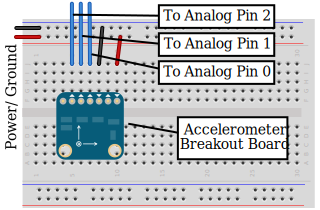
\includegraphics[width=\tw]{input-accel-annotated.svg.pdf}

  \vspace{0.0in}
  \begin{Verbatim}[gobble=3,fontsize=\small]
    int pin_x_accel = A0;
    int pin_y_accel = A1;
    int pin_z_accel = A2;

    // Calibration

    int xmin = 267; int xmax = 399;
    int ymin = 272; int ymax = 404;
    int zmin = 274; int zmax = 412;

    void setup() {
      Serial.begin(9600);
    }

    // Return average of 10 readings over 10ms
    int ReadAxis( int axisPin ) {
      long reading = 0;
      delay(1);
      for(int i = 0; i < 10; ++i)
        reading += analogRead( axisPin );
      return reading / 10;
    }
  \end{Verbatim}
\end{minipage}
\hfill
\begin{minipage}[t]{0.49\tw}
  \vspace{0.0in}
  \begin{Verbatim}[gobble=3,fontsize=\small]
    void loop() {
      // Read each axis.

      int x_raw = ReadAxis( pin_x_accel );
      int y_raw = ReadAxis( pin_y_accel );
      int z_raw = ReadAxis( pin_z_accel );

      // Scale measurements to calibrated minimum
      // and maximum.

      int x_scaled =
        map( x_raw, x_min, x_max, -1000, 1000 );
      int y_scaled =
        map( y_raw, y_min, y_max, -1000, 1000 );
      int z_scaled =
        map( z_raw, z_min, z_max, -1000, 1000 );

      // Report scaled measurements.

      Serial.print("x: ");
      Serial.print( x_scaled / 1000.0 );
      Serial.print("y: ");
      Serial.print( y_scaled / 1000.0 );
      Serial.print("z: ");
      Serial.print( z_scaled / 1000.0 );
      Serial.println();

      // Wait 500ms before next reading.

      delay(500);
    }
  \end{Verbatim}
\end{minipage}
\vspace{0.1in}

%Questions:
